\documentclass[border=4pt]{standalone}
\usepackage{amsmath,amssymb}
\usepackage{tikz}
\begin{document}
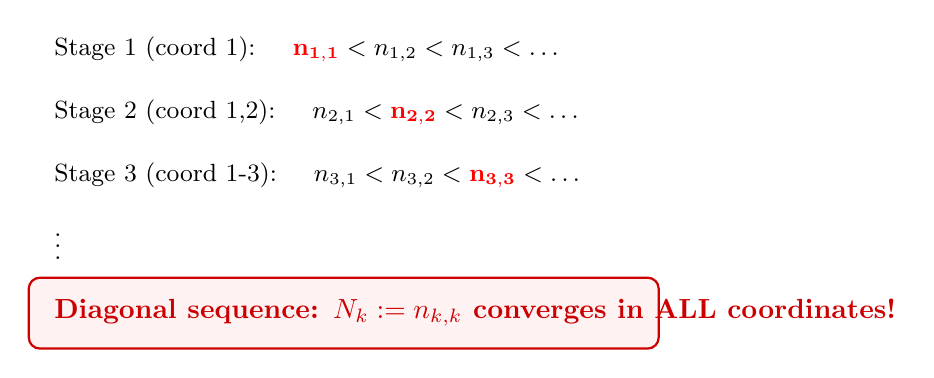
\begin{tikzpicture}[font=\small]
  \node[anchor=west] at (0, 3.0) {Stage 1 (coord 1): \quad $\mathbf{\color{red}n_{1,1}} < n_{1,2} < n_{1,3} < \dots$};
  \node[anchor=west] at (0, 2.2) {Stage 2 (coord 1,2): \quad $n_{2,1} < \mathbf{\color{red}n_{2,2}} < n_{2,3} < \dots$};
  \node[anchor=west] at (0, 1.4) {Stage 3 (coord 1-3): \quad $n_{3,1} < n_{3,2} < \mathbf{\color{red}n_{3,3}} < \dots$};
  \node[anchor=west] at (0, 0.6) {$\vdots$};
  \draw[thick, red!80!black, rounded corners=4pt, fill=red!5] (-0.2, -0.8) rectangle (7.8, 0.1);
  \node[anchor=west, font=\bfseries, text=red!80!black] at (0, -0.35) 
    {Diagonal sequence: $N_k := n_{k,k}$ converges in ALL coordinates!};
\end{tikzpicture}
\end{document}